\subsection*{F-measure and ROC-curve}
In a 10 times 10-fold crossvalidation, our predictor achieves an average F-max (the highest F-measure for any given confidence level) of $0.35\pm 0.03$ at a confidence level of $0.34$. Figure \ref{img:preRec_ROC} shows the precision recall and ROC curves averaged over the tenfolds of the crossvalidation. The sharp jumps in both curves are an artefact of jumps in the confidence function that clusters around few values for most predictions. In future releases of HypfuNN we hope to achieve a smoother confidence score with optimized activation functions in the output layer of the neural network.

\begin{figure}[!h]
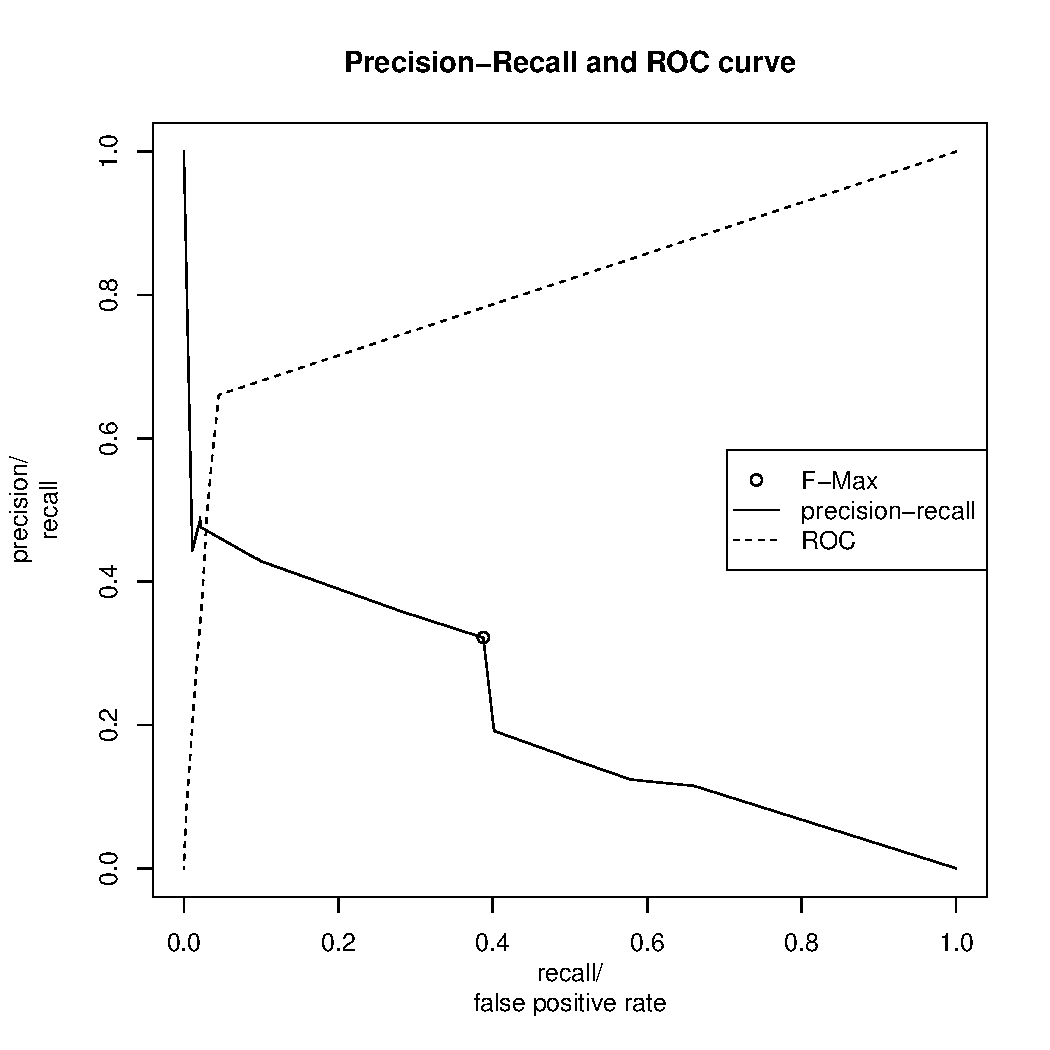
\includegraphics[width=0.45\textwidth]{figures/PreRecROC.pdf}
\caption{Precision-Recall curve (solid line) of HypfuNN predictions. The best F-measure is achieved at confidence $0.34$ with precision $0.32 \pm 0.04$ and recall $0.39 \pm 0.10$. The second set of axes and dashed line describe the ROC curve of HpyfuNN predictions.}
\label{img:preRec_ROC}
\end{figure}

\subsection*{Predictions for Human Proteome}

For 20231 human protein sequences provided the CAFA challenge, our predictor provides 3.9 mio HPO-terms with a confidence larger than $0.34$, the threshold for our F-max value. These predictions are reduced to the most specific terms with equal confidence, i.e.~a parent node that is predicted with an equal confidence as a child, it is not counted separately. Assuming our error measures hold in general, we add 1.2 mio correct functional annotations to largely not yet described protein sequences. On the flipside, we also add many false annotations, although it can be expected that some of them lead in the right direction. For example if we incorrectly predict a HPO term, but the parent of this term is correct, then our prediction is strictly counted only as false positive, but still could give a valuable lead to the proteins correct function.